\subsubsection*{Guided Filter}

Für die Anwendung des Guided Filters wurde, wie bereits erwähnt, die Computer Vision Bibliothek OpenCV verwendet. Um diesen Filter mit OpenCV anwenden zu können mussten zuvor das RGB Bild und das Tiefenbild in das OpenCV Format gebracht werden. Dies war jedoch mit den Methoden \enquote{glReadPixels} und \enquote{glTexImage2D} für den aktuell selektierten Framebuffer und der OpenGL Textur problemlos möglich. Zwar sind die Speicherkonventionen von OpenGL und OpenCV, was die X und Y Achse angeht, genau vertauscht, jedoch ist das Filtern, welches daraus folgend gedreht stattfindet, für den Nutzer völlig intransparent und muss nicht weiter berücksichtigt werden.\\

Problematisch ist jedoch, dass das OpenGL Tiefenbild eine Farbtiefe von 16Bit nutzt und der OpenCV Guided Filter nur auf 8Bit Graustufen angewendet werden kann. Diese Transformation und die daraus resultierende Ungenauigkeit der Tiefe wurde jedoch zunächst in Kauf genommen, da erst einmal der Mechanismus als solches getestet werden soll. In der späteren Auswertung von Testszenarien muss diese Transformation berücksichtigt werden. \\

Diese Implementierung ermöglicht es, den Guided Filter dynamisch auf das aktuell generierte Tiefenbild mit dem aktuell aufgenommen RGB Bild als Leitbild anzuwenden. Außerdem lassen sich die Filter Parameter, dem Radius \(r\) und den Einflussfaktor \(\epsilon\) dynamisch variieren. Abbildung \ref{fig:filter-demo} zeigt das Tiefenbild der TSDF Rekonstruktion links, auf die rechts der Guided Filter mit dem aktuellen RGB Bild angewendet wurde. \\

\begin{figure}[h]
  \centering
	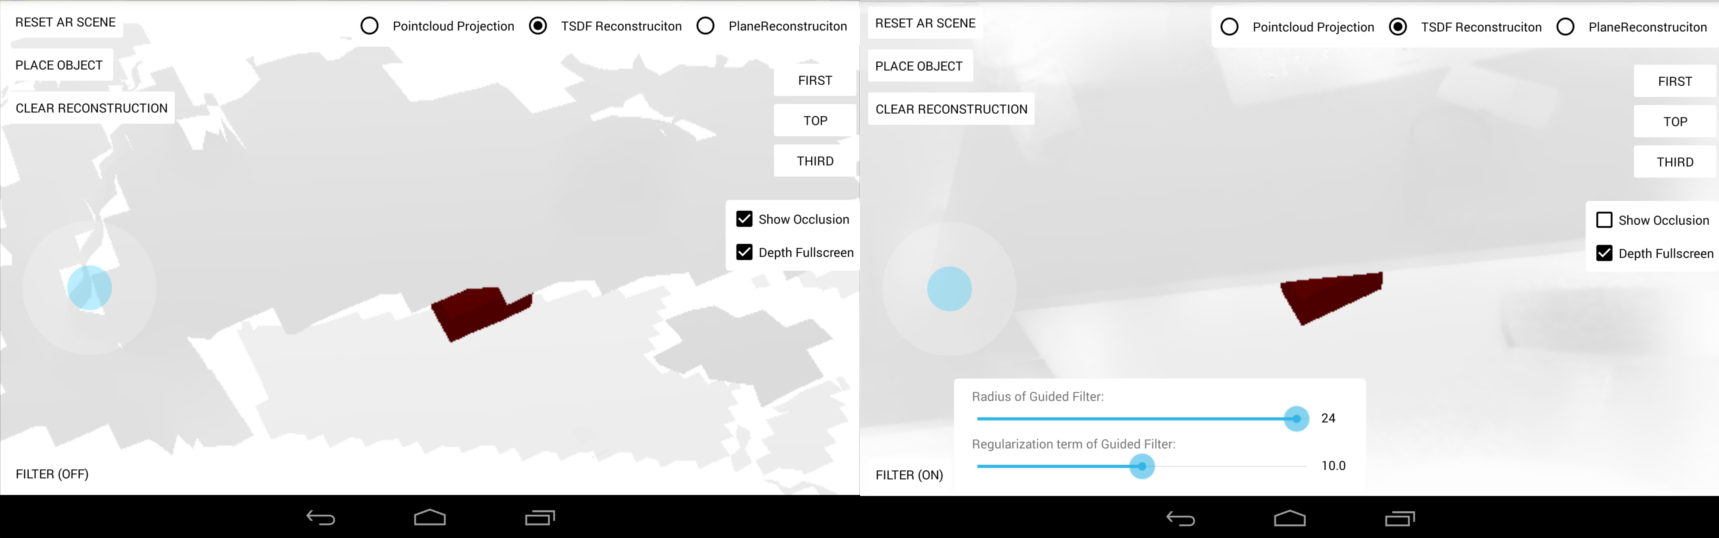
\includegraphics[width=1.0\textwidth]{content/images/implementation/filter-demo.png} 
  \caption{Anwendung des Guided Filters auf eine TSDF Rekonstruktion. Links vor und rechts nach der Anwendung.}
  \label{fig:filter-demo}
\end{figure}
